%\documentclass[11pt,professionalfonts,hyperref={pdftex,pdfpagemode=none,pdfstartview=FitH}]{beamer}
%\usepackage{times}
\documentclass[11pt,professionalfonts]{beamer}
\usefonttheme{serif}

\usepackage{aas_presentation_packages}
\bibliography{library} % must be in the preamble when using biblatex package

\DeclareSIUnit\year{yr}

\newcommand{\vs}{\vspace{0.3cm}}

\definecolor{mygray}{gray}{0.9}
\definecolor{RoyalBlue}{rgb}{0.25,0.41,0.88}
\def\Emph{\textcolor{RoyalBlue}}

\definecolor{tmp}{rgb}{0.804,0.941,1.0}
\setbeamercolor{numerical}{fg=black,bg=tmp}
\setbeamercolor{exact}{fg=black,bg=red}

\mode<presentation> 
{
  \usetheme{Warsaw}
  \usefonttheme{serif}
  \setbeamercovered{transparent}
}

\setbeamertemplate{footline}%{split theme}
{%
  \leavevmode%
  \hbox{\begin{beamercolorbox}[wd=.5\paperwidth,ht=2.5ex,dp=1.125ex,leftskip=.3cm,rightskip=.3cm plus1fill]{author in head/foot}%
    \usebeamerfont{author in head/foot}\insertshorttitle
  \end{beamercolorbox}%
  \begin{beamercolorbox}[wd=.5\paperwidth,ht=2.5ex,dp=1.125ex,leftskip=.3cm,rightskip=.3cm]{title in head/foot}
%    \usebeamerfont{title in head/foot}\mypaper\hfill \insertframenumber/\inserttotalframenumber
    \usebeamerfont{title in head/foot}\hfill \insertframenumber/\inserttotalframenumber
  \end{beamercolorbox}}%
  \vskip0pt%
} \setbeamercolor{box}{fg=black,bg=yellow}


\title[Reachability Sets on \Poincare section]{\large\bf  Low-Thrust Trajectory Design Using Reachability Sets near Asteroid 4769 Castalia}

\author{\vspace*{-0.3cm}}

   
\institute{
  \footnotesize
  {\normalsize\bf{Shankar Kulumani and Taeyoung Lee}}\\
  \vspace*{0.2cm}
    \textbf{Flight Dynamics \& Control Lab}\\ \vspace*{0.5cm}
  \begin{figure} %figure%
        
\includegraphics[width=0.75\textwidth]{gw_txh_2cs_pos}
    \end{figure}
}
\date{}

\begin{document}
%=======================================================%

\setcounter{framenumber}{-1}
\begin{frame} %-----------------------------%
  \titlepage
\end{frame}   %-----------------------------%

\section*{Introduction}
\subsection*{Motivation}  

\begin{frame}{Asteroid Missions}
\begin{itemize}
    \item Science - insight into the early formation of the solar system
    \item Mining - vast quantities of useful materials
    \item Impact - huge threat to humanity from impact
\end{itemize}    

\begin{center}
    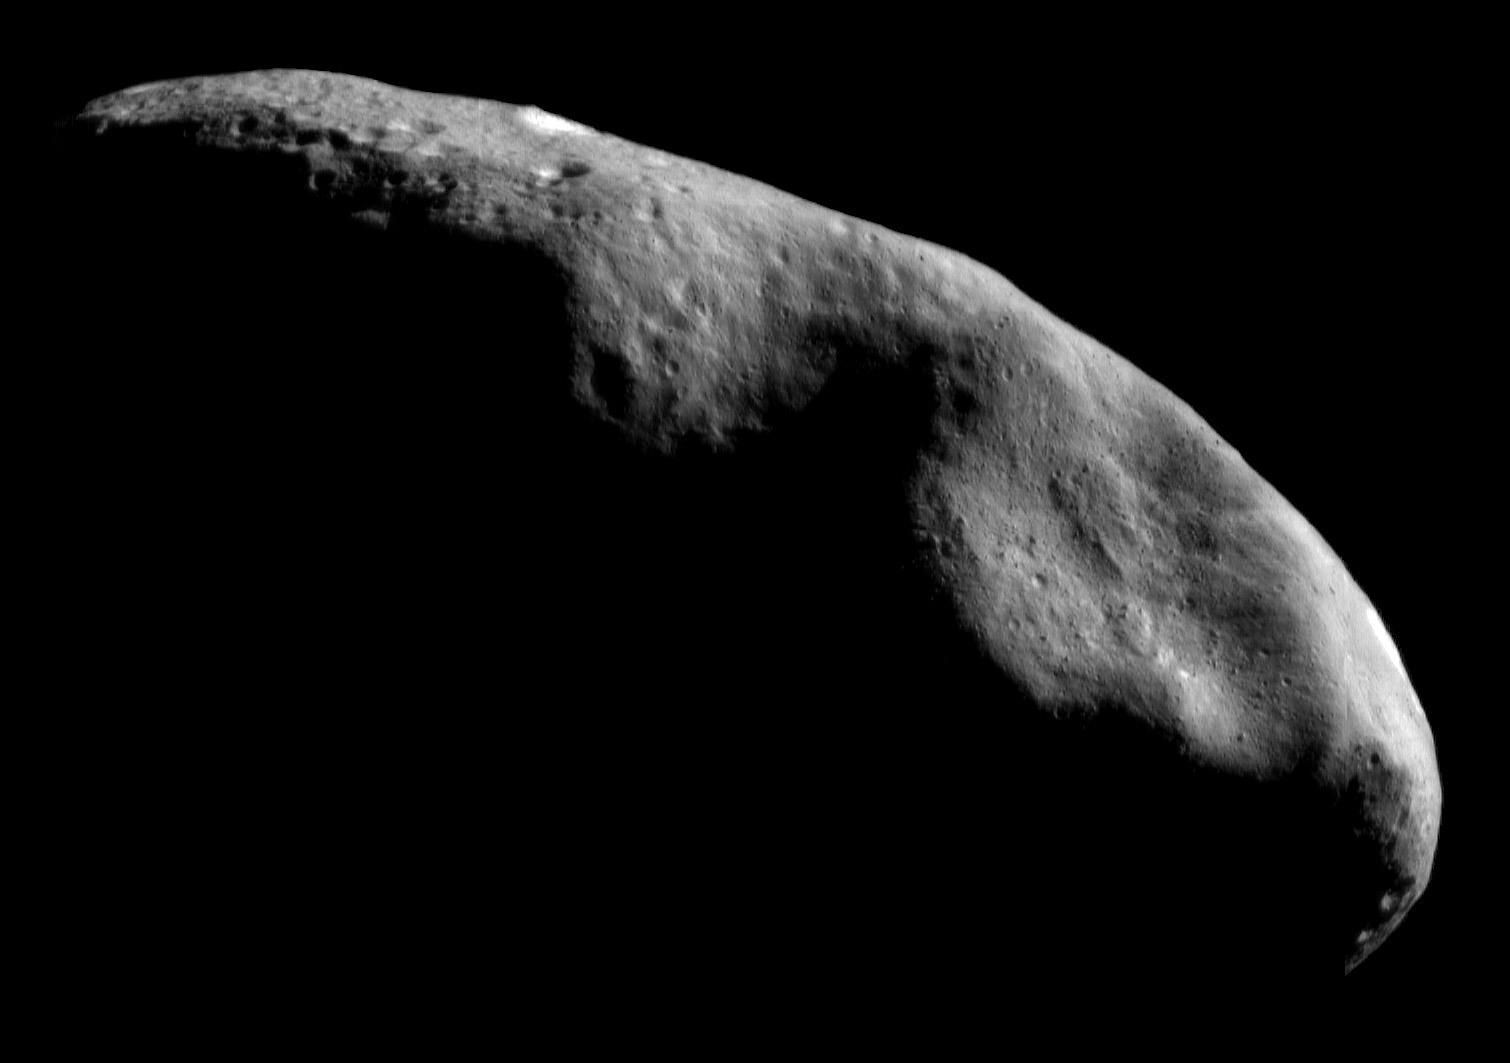
\includegraphics[height=0.35\textheight]{figures/near_mos_20001203_full.jpg}
    \hfill
    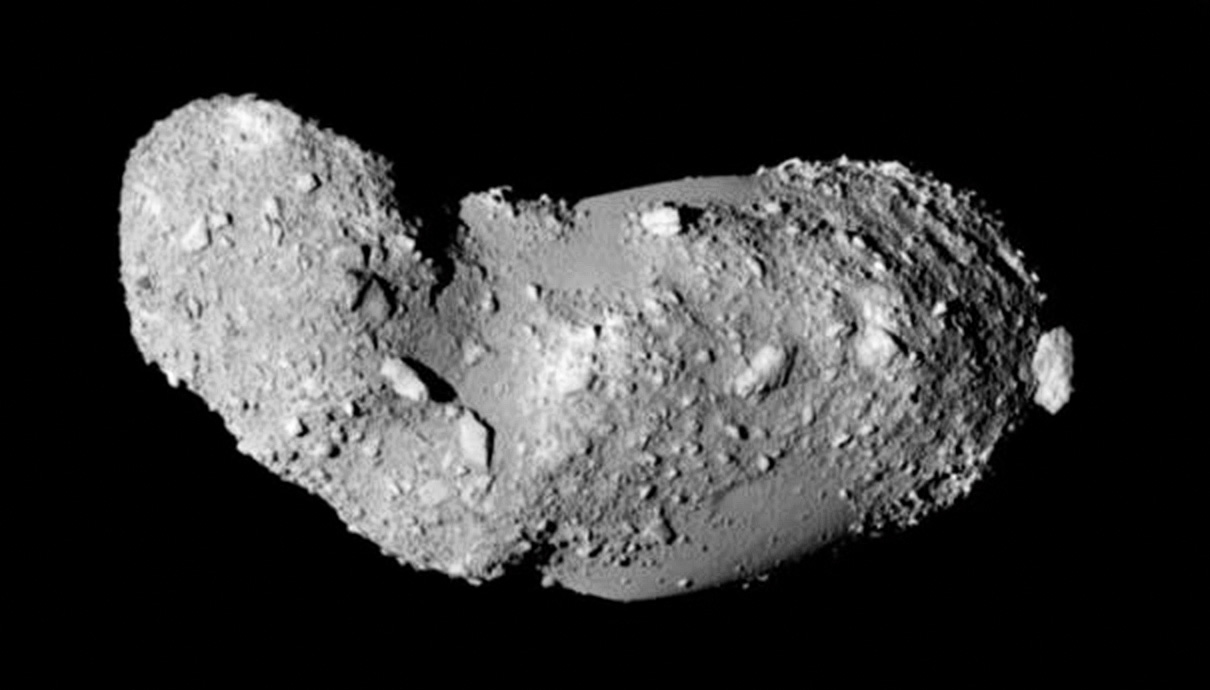
\includegraphics[height=0.35\textheight]{figures/Itokawa8_hayabusa_1210.jpg}
\end{center}
\end{frame}

\begin{frame}{Asteroid Mining}
    \begin{itemize}
      \item Useful materials can be extracted from asteroids to support:
      \begin{itemize}
          \item Propulsion, construction, life support, agriculture, and precious/strategic metals
      \end{itemize}
      \item Commercialization of near-Earth asteroids is feasible~\footfullcite{ross2001}
    \end{itemize}

\begin{center}
\small
    \begin{tabular}{|l|r|r|}
        \hline 
        Element & Price (\SI{}{\$\per\kilo\gram}) & Sales (\SI{}{\$M\per\year}) \\
        \hline \hline 
        Phosphorous (P) & \num{0.08}  & \num{2167} \\
        Gallium (Ga) & \num{300.00}  & \num{1544} \\
        Germanium (Ge) & \num{745.00} & \num{6145} \\
        \hline \hline 
        Platinum (Pt) & \num{12394.00} & \num{1705} \\
        Gold (Au) & \num{12346.00} & \num{49} \\
        Osmium (Os) & \num{12860.00} & \num{307} \\
        \hline
    \end{tabular}
\end{center}

\end{frame}


\begin{frame} %-----------------------------%
\frametitle{Low-thrust vehicles} % electric propulsion
\begin{itemize}
    \item Low-thrust orbital transfers
    \begin{itemize}
        \item Electric propulsion has increased in popularity
        \item Offers much higher specific impulse than chemical engines 
        \item Requires much longer operating periods for maneuvers 
        \item Enables long duration missions with frequent thrusting
    \end{itemize}
\end{itemize}

\begin{center}
    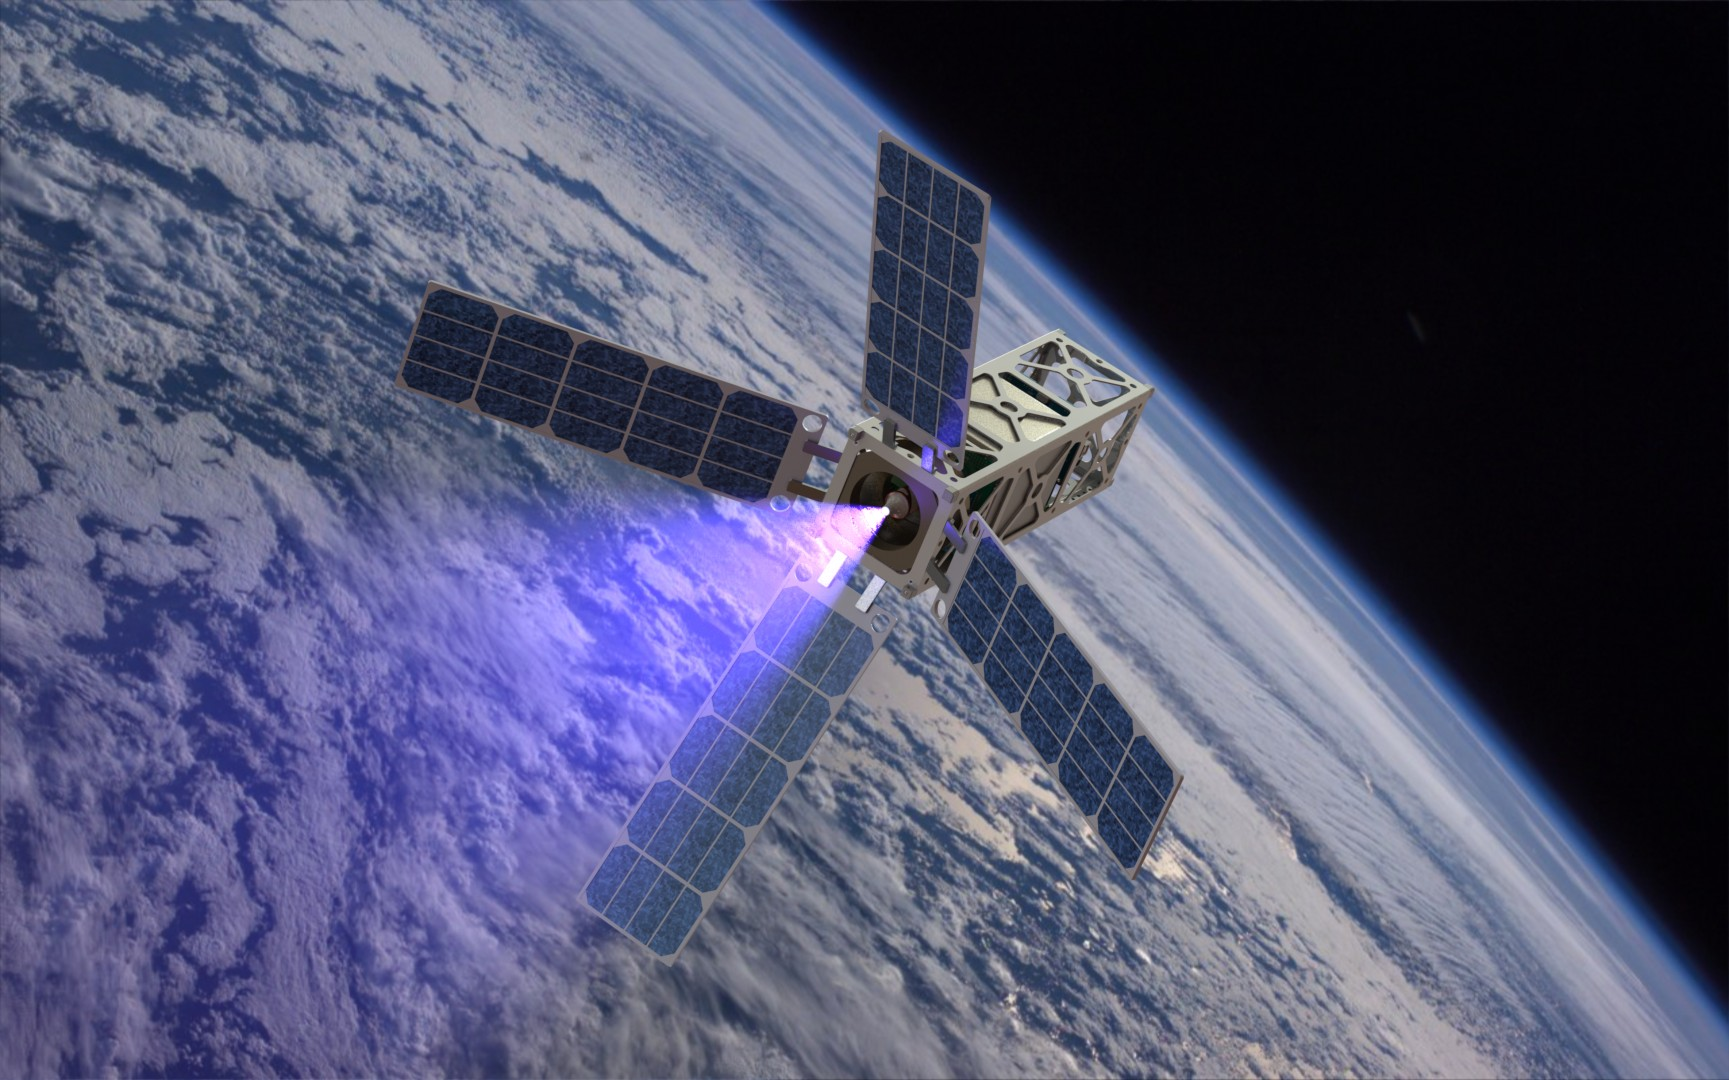
\includegraphics[height=0.3\textheight]{patriot_plume}
    \hfill
    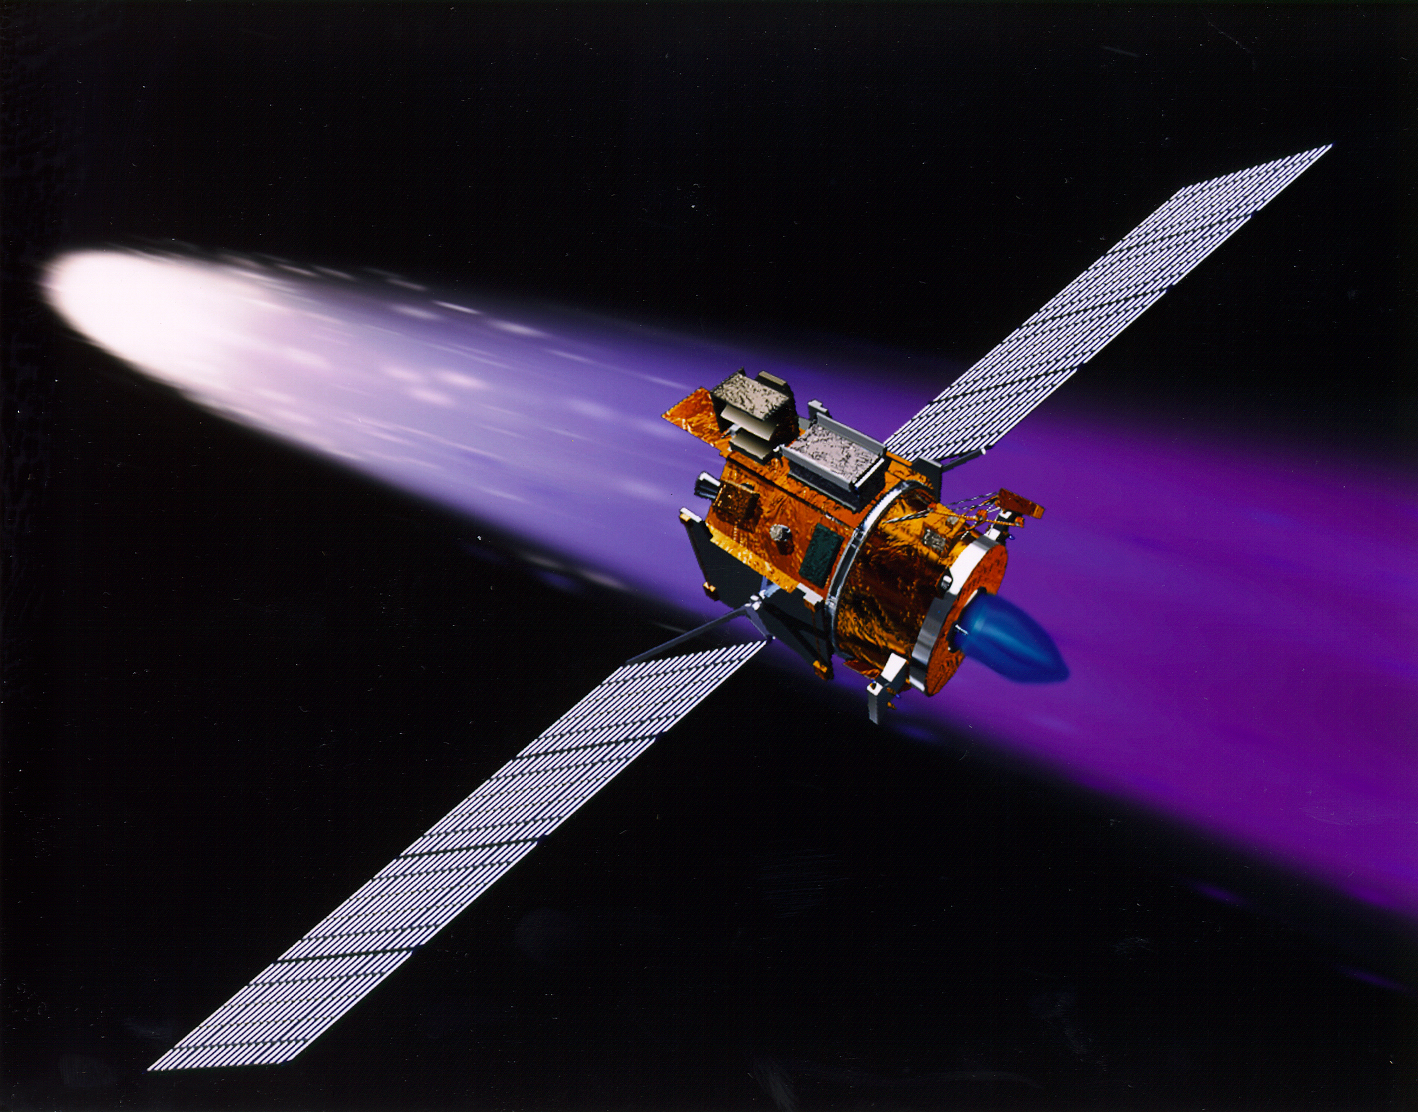
\includegraphics[height=0.3\textheight]{deepspace1}
\end{center}
\end{frame}   %-----------------------------%

\section*{Previous Work}
\subsection*{Past Challenges}

\begin{frame}{Gravitational Modeling} %-----------------------------%

\begin{itemize}
  \item Asteroids are extended bodies not point masses
  \item Spherical Harmonic - popular, but only valid outside of circumscribing sphere
    {
    \small
    \begin{align*}
      U(\vecbf{r} ) = \frac{\mu}{r} \sum_{n=0}^\infty \sum_{m=0}^\infty \parenth{\frac{R}{r}}^nP_{n,m}(\sin \phi) \braces{ C_{nm} \cos(m \lambda) + S_{nm} \sin(m \lambda)} 
    \end{align*}
    }
  \item Infinite series is always an approximation and adds complexity
    \begin{itemize}
        \item Model switching at circumscribing sphere
        \item Coefficient matching to ensure continuity across switching region
    \end{itemize}
\end{itemize}

\note[itemize]{
  \item Models require detailed data from orbit about asteroid (OD process determines gravity field)
  \item Simplified models (triaxial ellipsoid allows analytical insight)
  \item Previous work fails to consider coupled dyanmics
  }

\end{frame}   %-----------------------------%

\begin{frame}{Optimal Transfers} %-----------------------------%

\begin{itemize}
    \item Optimal Trajectory Design
        \begin{itemize}
            \item Orbital dynamics are nonlinear and chaotic
            \item Very sensitive to initial conditions
            \item Intuition required by designer to enable convergence
        \end{itemize}
    \pause
    \item Direct Optimal Control
        \begin{itemize}
            \item Reformulate problem as parameter optimization
            \item Allows for use of nonlinear programming methods
            \item High dimensional problem and computationally intensive
            \item Results in suboptimal solutions due to discretization
        \end{itemize}
\end{itemize}
\end{frame}   %-----------------------------%

\section*{Research Approach}
\subsection*{System Model}

\begin{frame}{Polyhedron Gravitation Model}

\begin{itemize}
    \item Compute potential assuming faceted shape model of asteroid
    \item Globally valid, closed-form expression of potential
    \item Exact potential assumes a constant density and an accurate shape model
\end{itemize}
\only<2>{
\begin{align*}\label{eq:potential}
    U(\vecbf{r}) &= \frac{1}{2} G \sigma \sum_{e \in \text{edges}} \vecbf{r}_e \cdot \vecbf{E}_e \cdot \vecbf{r}_e \cdot L_e - \frac{1}{2}G \sigma \sum_{f \in \text{faces}} \vecbf{r}_f \cdot \vecbf{F}_f \cdot \vecbf{r}_f \cdot \omega_f \in \R^1
\end{align*}
}
\only<3>{
\begin{center}
  \animategraphics[autoplay,loop,width=0.5\textwidth]{30}{./animation/castalia/castalia-}{0}{999}~\hfill
  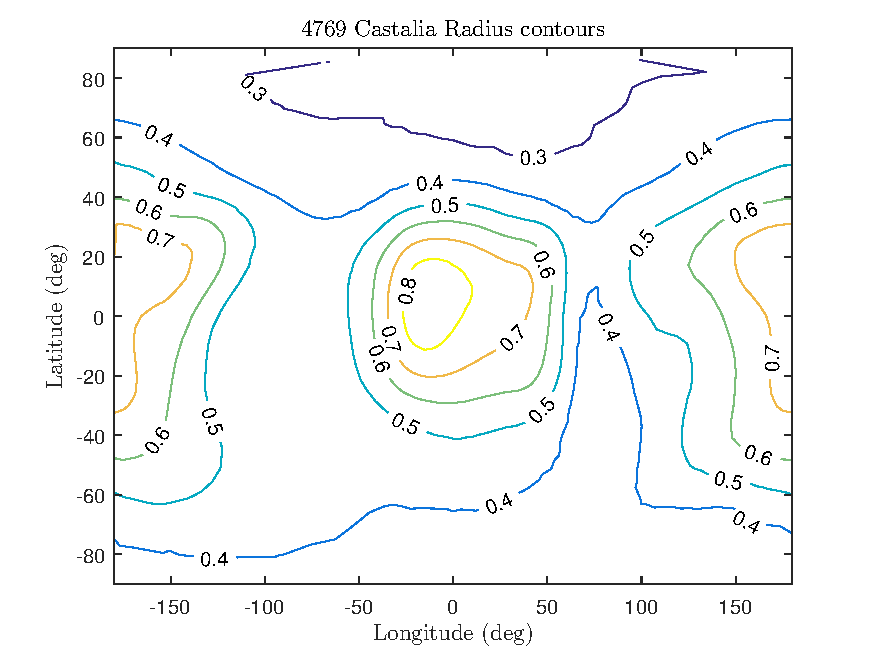
\includegraphics[width=0.5\textwidth]{figures/radius_contour.pdf}
\end{center}
}

\end{frame}

\begin{frame}{Equations of Motion}

\begin{itemize}
    \item Many similarities to the three-body problem
    \item Much of the same theory is also applicable
\end{itemize}

\begin{align} \label{eq:eoms}
    \begin{split}
        \ddot{x} - 2 \omega \dot{y} - \omega^2 y &= U_x , \\
        \ddot{y} + 2 \omega \dot{x} - \omega^2 x &= U_y , \\
        \ddot{z} &= U_z .
    \end{split}
\end{align}
\pause
\begin{itemize}
    \item Dynamics allow for a single integral of motion
\end{itemize}

\begin{align}\label{eq:jacobi}
    J \parenth{\vecbf{r}, \vecbf{v}} = \frac{1}{2} \omega^2 \parenth{x^2 + y^2} + U(\vecbf{r}) - \frac{1}{2} \parenth{\dot{x}^2 + \dot{y}^2 + \dot{z}^2} .
\end{align}

\end{frame}


\subsection*{Proposed Approach}

\begin{frame}{Proposed Approach} % -----------------------------------%
  \begin{itemize}
      \item Extend invariant manifold concept with low-thrust control  
      \item Variational integrator allows for accurate and stable computation
      \item \emph{Computational geometric optimal control} used to generate reachable set
      \item \emph{Reachability set} on Poincar\'e section allows for systematic transfer design
  \end{itemize}
\end{frame} %--------------------------------------%

\begin{frame}{\Poincare map}
\begin{itemize}
    \item Intersection of a periodic orbit with a lower dimensional subspace, \Poincare section
    \item Useful for investigating the stability and structure of dynamical systems
    \item We define a section \( \Sigma \) to determine initial and target periodic orbits for our transfer
\end{itemize}

\begin{align}\label{eq:poincare_section}
    \Sigma = \braces{\parenth{x, \dot{x}, z, \dot{z}} | y(t_f) = 0 }.
\end{align}

\end{frame}

\begin{frame}{Reachability Set}

\begin{itemize}
    \item Set of states achievable from a given initial condition over fixed \( t_f \) s.t. maximum control contraint
    \[
    R( \vecbf{x}_0, \mathcal{U} , t_f) = \braces{ \vecbf{x}_f \subseteq \mathcal{X} | \exists \vecbf{u} \in \mathcal{U}, \vecbf{x}(t_f) = \vecbf{x}_f }
    \]
    \item Directly derivable from optimal control
    \item Frequently used for safety planning, e.g. air traffic collision avoidance
    \item We extend its use to the design of spacecraft transfers
\end{itemize}

\end{frame}

\begin{frame}{Reachability Set on \Poincare section} % -----------------------------------%

\begin{itemize}
    \item We seek to generate the reachability set on a chosen \Poincare section
    \[
        \Sigma = \braces{\parenth{x, \dot{x}, z, \dot{z}} | y(t_f) = 0 }.
    \]
    \item Control input is chosen to enlarge the reachable set
\end{itemize}
\pause
\begin{figure}
    \centering
    \begin{scaletikzpicturetowidth}{0.3\textwidth}
    \begin{tikzpicture}[scale=\tikzscale]
        \coordinate [label=left:\textcolor{black}{\large \(\vecbf{x}_0\)}] (x0) at (-1,-2);
        \coordinate [label=below:\textcolor{black}{\large  \(\vecbf{x}_n\)}] (xn) at (1,1);
        \coordinate [label=left:\textcolor{black}{\large  \(\Sigma\)}] (sigma) at (-4,3);
        %\coordinate [label=below:\textcolor{black}{\large  \(P(\vec{x})\)}] (P) at (0,-3.5);
        % define the path of the flow with coordinates
        \coordinate [label=right:\textcolor{black}{}] (f1) at (5,-2);
        \coordinate [label=below:\textcolor{black}{\large  \(\psi(t,\vecbf{x}_0)\)}] (f2) at (2,-5);
        \coordinate [label=right:\textcolor{black}{}] (f3) at (-4,-4);
        \coordinate [label=right:\textcolor{black}{}] (f4) at (-4,-1);
        
    %   \draw[help lines] (-10,-10) grid (10,10); %grid
        \filldraw [black] (x0) circle [radius=3pt];
        \filldraw [black] (xn) circle [radius=3pt];
    
        \draw [ultra thick,black,->-](x0) to[out=20,in=90,distance=2cm] (f1) to[out=-90,in=0,distance=2cm] (f2) to[out=180,in=-45,distance=2cm] (f3) to[out=135,in=-135,distance=2cm] (f4) ;
        \draw [ultra thick, black,dashed,->] (f4) to[out=45,in=180,distance=1cm] ($(xn)-(2,0)$);
        
        \draw [ultra thick] plot [smooth cycle, tension=0.1, rotate=5] coordinates { (-4,-3) (4,-3) (4,3) (-4,3) };
    
        \draw [thick,dashed] (xn) circle [radius=2cm]; % reachability set
    
        \draw [thick,->] (xn) -- ($(xn) + (2.5,0)$);
        \draw [thick,rotate=45,->] (xn) -- ($(xn) + (2.5,0)$);
        \draw ($(xn) + (1,0)$) arc [start angle=0,end angle=45, radius=1];
        \node [draw=none] at (2.4,1.5) {\Large \(\phi_d\)};
        \draw [decorate,decoration={brace,amplitude=5pt},rotate=45] (xn) -- ($(xn) + (2,0)$);
        \node [draw=none] at ($ (xn) + (0,1) $) {\Large \( J \)};
    \end{tikzpicture}
    \end{scaletikzpicturetowidth}
\end{figure}

\end{frame} %--------------------------------------%

\begin{frame}{Optimal Control Problem}
\begin{itemize}
    \item Reachability defined as distance between controlled and uncontrolled states
    \begin{align}\label{eq:cost}
        J = -\frac{1}{2} \left( \vecbf{x}(t_f) - \vecbf{x}_{n}(t_f)\right)^T 
        Q
        \left( \vecbf{x}(t_f) - \vecbf{x}_{n}(t_f)\right) ,
    \end{align}
    \item Terminal constraints used to ensure correct section and specific direction on \( \R^4 \)
        \begin{align}\label{eq:terminal_constraints}
            \begin{split}
                m_1 &= y = 0 , \\
                m_2 &= \parenth{\sin \phi_{1_{d}}} \parenth{ x_1^2 + x_2^2 + x_3^2 + x_4^2} - x_1^2 = 0, \\
                m_3 &= \parenth{\sin \phi_{2_{d}}} \parenth{ x_2^2 + x_3^2 + x_4^2} - x_2^2 = 0, \\
                m_4 &= \parenth{\sin \phi_{3_{d}}} \parenth{ 2 x_3^2 + 2 x_3 \sqrt{x_4^2 + 2 x_4^2}} - x_3 - \sqrt{x_4^2 + x_3^2} = 0 ,
            \end{split}
        \end{align}
    \item Maximum acceleration bound to emulate realistic system
        \begin{align}\label{eq:control_constraint}
            c(\vecbf{u}) = \vecbf{u}^T \vecbf{u} - u_m^2 \leq 0 ,
        \end{align}
\end{itemize}

\end{frame}

\begin{frame}{Terminal Constraints}
Constraint for section

Constraints for direction

Constraint for control
\end{frame}

\section*{Transfer Example}
\subsection*{Numerical Simulation}

\begin{frame}{Simulation} %-----------------------------%

Describe transfer example

Show animation in both body and inertial frame

Show reachability set

% \animategraphics[autoplay,loop,width=0.5\textwidth]{8}{./animation/single_noavoid/single_noavoid-}{0}{99}~
% \animategraphics[autoplay,loop,width=0.5\textwidth]{8}{./animation/single_avoid/single_avoid-}{0}{99}

\end{frame}%-----------------------------%


\section*{}
\subsection*{}

\begin{frame}{Conclusions} %-----------------------------%

  

\end{frame}   %-----------------------------%

\begin{frame}[c]{Thank you}
  \centering
  
  \textbf{\large Flight Dynamics \& Control Lab} \\
  Mechanical \& Aerospace Engineering \\
  School of Engineering \& Applied Science
  
  \begin{figure} %figure%
        
\includegraphics[width=0.75\textwidth]{gw_txh_2cs_pos}
    \end{figure}
  
  \url{https://fdcl.seas.gwu.edu}
\end{frame}

\end{document}

